\section{HPA darba punkta iestatīšana/atiestatīšana}
Darba punkta noteikšanai (skat. 3.1. att.) tika mērīta noteces strāva , 12  un 24 V industriālā barošanas avota līnijas, ieslēgšanas/izslēgšanas slēdža vadības signāls un RF jaudas pastiprinātāja aizvara spriegums. Noteces strāva jaudas pastiprinātājam tiek mērīta ar multimetru, bet pārējie sistēmas parametri - ar osciloskopu.
\begin{figure}[H]
	\centering
    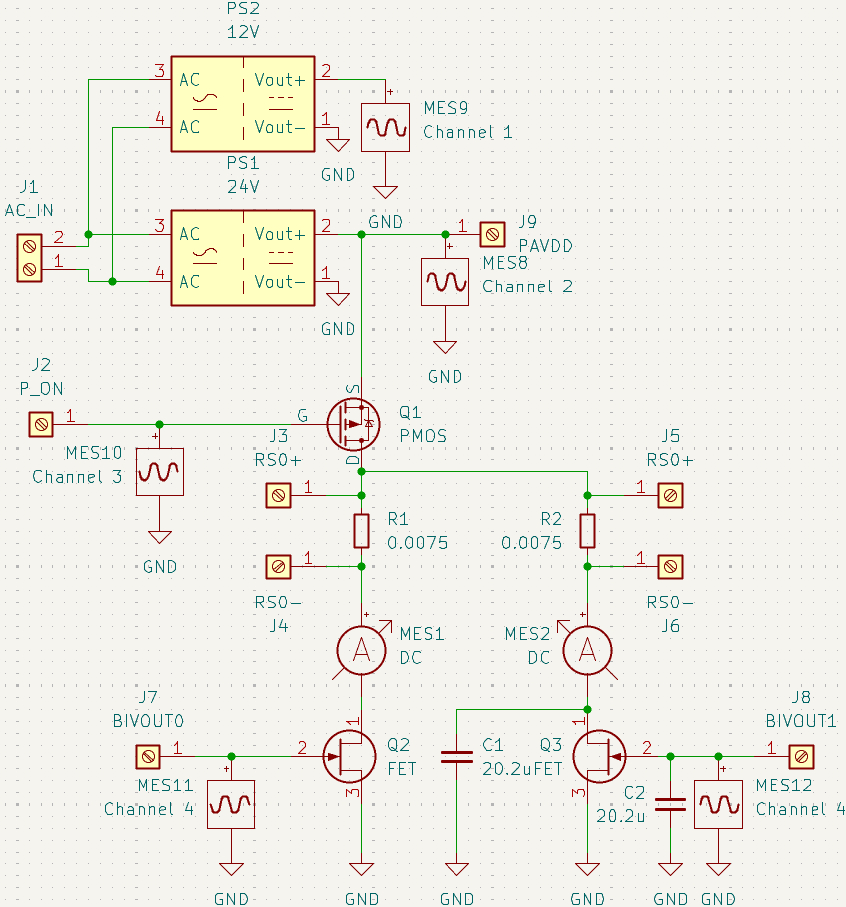
\includegraphics[width=0.8\textwidth]{pictures/test_diagram.png}\hspace{1cm}
    \caption{Darba punkta iestatīšanas/atiestatīšanas testa diagramma}
\end{figure}
Visās oscilogrammās 1. kanāls ir 12 V līnija, 2. kanāls ir 24 V līnija, 3. kanāls ir ieslēgšanas/izslēgšanas vadības signāls un 4. kanāls ir RF jaudas pastiprinātāja aizvara spriegums.
\begin{figure}[H]
	\centering
    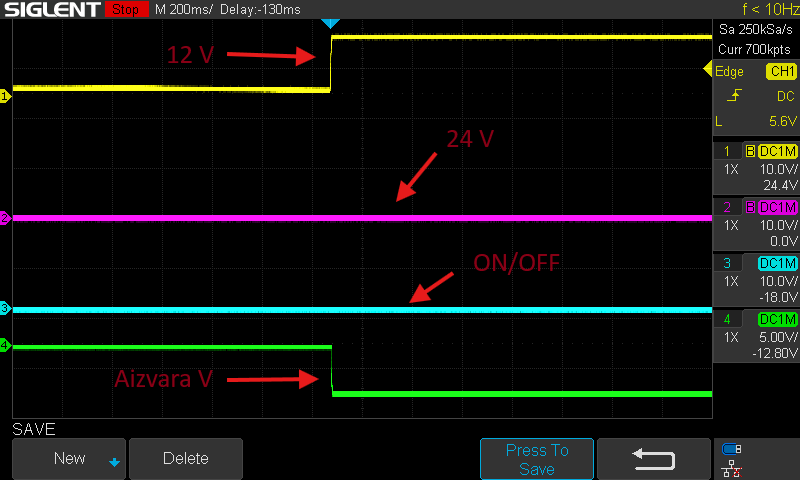
\includegraphics[width=0.9\textwidth]{pictures/device_startup.png}\hspace{1cm}
    \caption{Sistēmas ieslēgšana}
\end{figure}
 3.2. att. ieslēdzoties sistēmai, tiek ieslēgts 12 V barošanas avots, kas nodrošina jaudu visiem 9 V un 5 V patērētājiem, tālāk jaudas pastiprinātāja aizvara spriegums tiek iestatīts uz -5 V, lai to aizvērtu. 24 V barošanas avots netiek ieslēgts, jo to dara  mikrokontrolleris ar manuālu vai tīkla komandu, tāpēc arī nevar novērot 24 V vadības spriegumu ieslēgšanas/izslēgšanas slēdzim.
\begin{figure}[H]
	\centering
    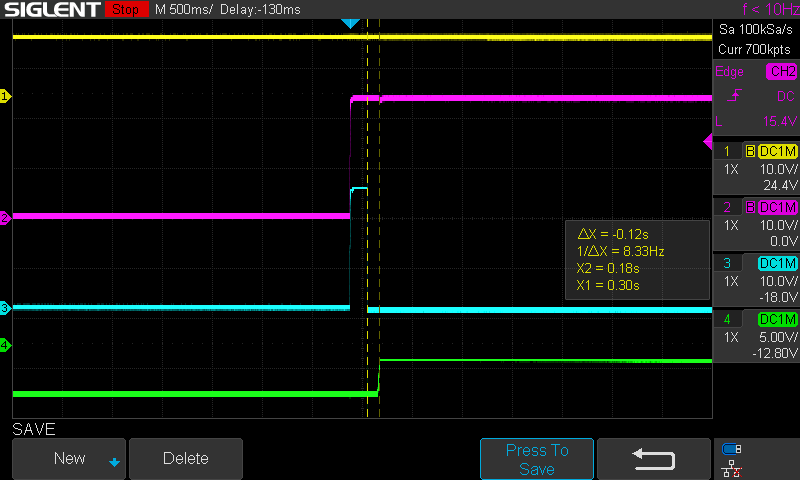
\includegraphics[width=0.9\textwidth]{pictures/load_nocap.png}\hspace{1cm}
    \caption{Sistēmas ieslēgšanās oscilogramma ar testa lauktranzistoru}
\end{figure}
\begin{figure}[H]
	\centering
    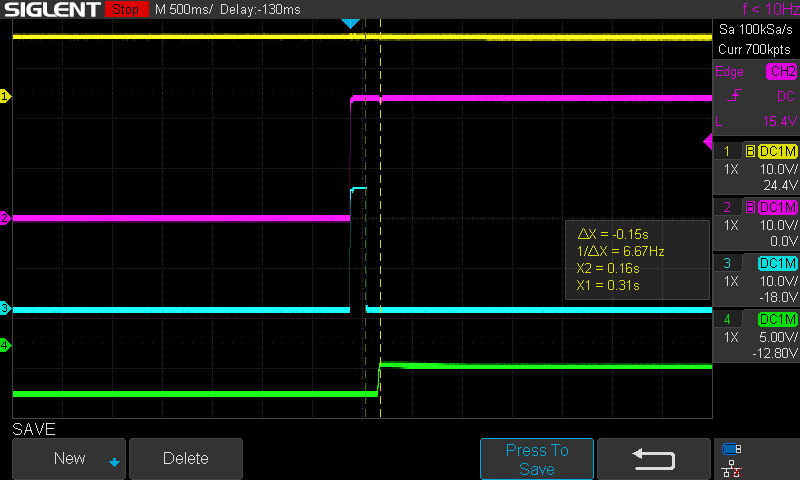
\includegraphics[width=0.9\textwidth]{pictures/capacitive_load.png}\hspace{1cm}
    \caption{Sistēmas ieslēgšanās oscilogramma ar testa lauktranzistoru un filtra kondensatoru}
\end{figure}
3.3. un 3.4. attēlā var redzēt darba punkta iestatīšanu, kur 3.4 attēlā tiek simulēts pats RF pastiprinātājs, pieliekot klāt kondensatorus filtrs. Kad tiek saņemta starta komanda mikrokontrollerī, tad tiek ieslēgts 24 V barošanas avots, kur momentā tiek nodrošināts aizvara spriegums ieslēgšanas/izslēgšanas p-kanāla lauktranzistoram, lai tas būtu aizvērtā stāvoklī. Tad pēc pāris milisekundēm tiek atvērts lauktranzistors un pēc datu lapas nodrošināta vismaz 100 milisekunžu aizture pēc p-kanāla lauktranzistora aktivizēšanas, lai nostabilizētos pārējie procesi.
\begin{figure}[H]
	\centering
    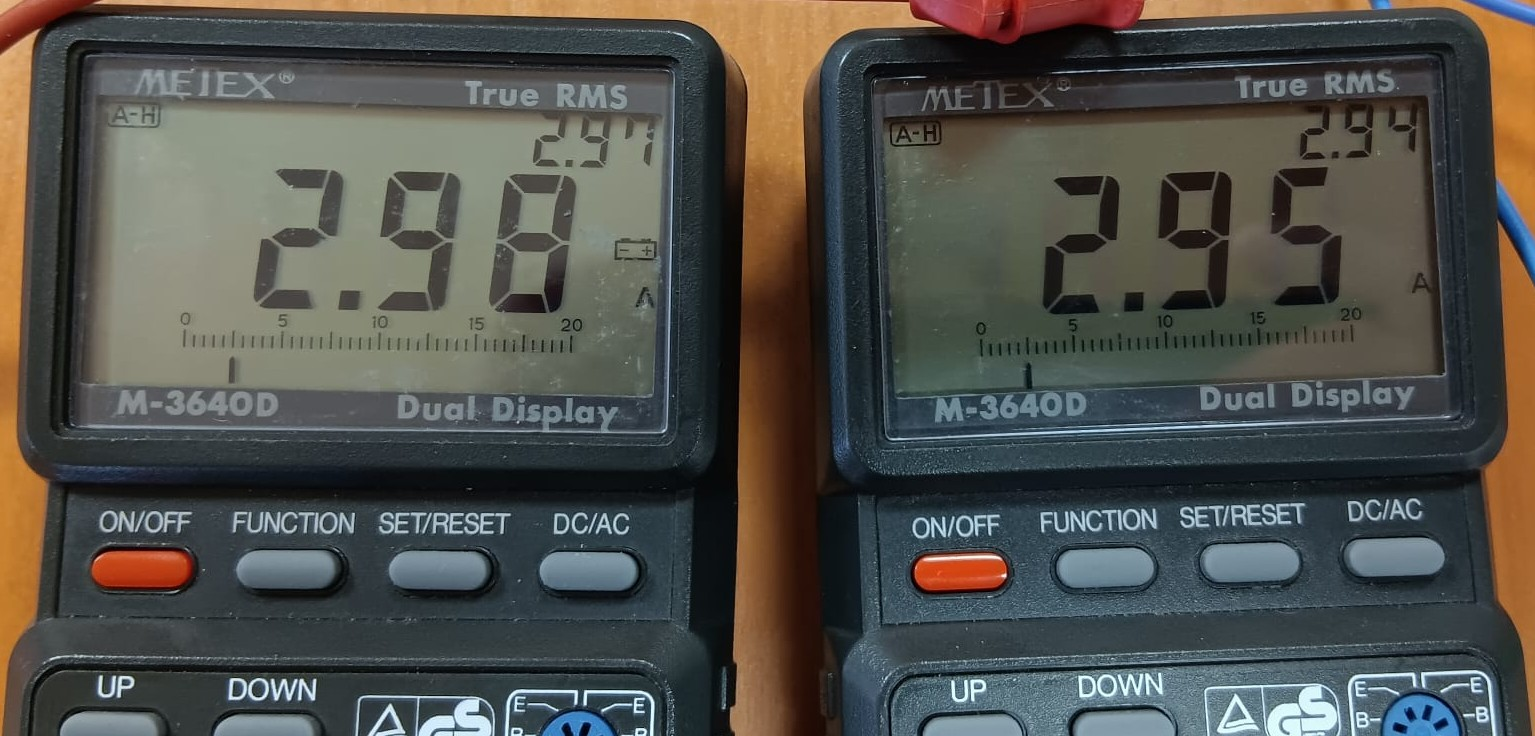
\includegraphics[width=0.9\textwidth]{pictures/load1load2_f.jpg}\hspace{1cm}
    \caption{Noteces strāvas kreisajam un labajam plecam RF jaudas pastiprinātājam}
\end{figure}
3.5. attēlā var redzēt noteces strāvas abiem RF jaudas pastiprinātāja pleciem. Kreisajā pusē 2.98 A tiek nodrošināti testa tranzistoram bez kapacitatīvas slodzes un labajā pusē 2.95 A ar kapacitatīvu slodzi, kas simulē RF jaudas pastiprinātāju.
\begin{figure}[H]
	\centering
    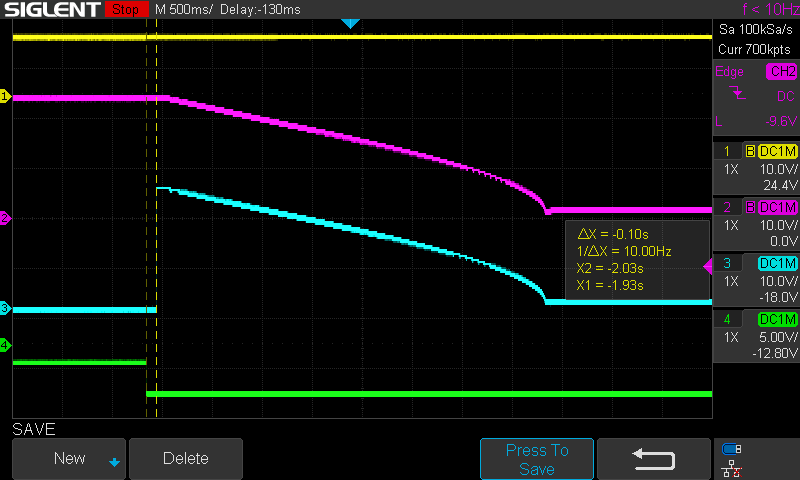
\includegraphics[width=0.9\textwidth]{pictures/load_off_nocap.png}\hspace{1cm}
    \caption{Sistēmas izslēgšana oscilogramma ar testa lauktanzistoru}
\end{figure}
\begin{figure}[H]
	\centering
    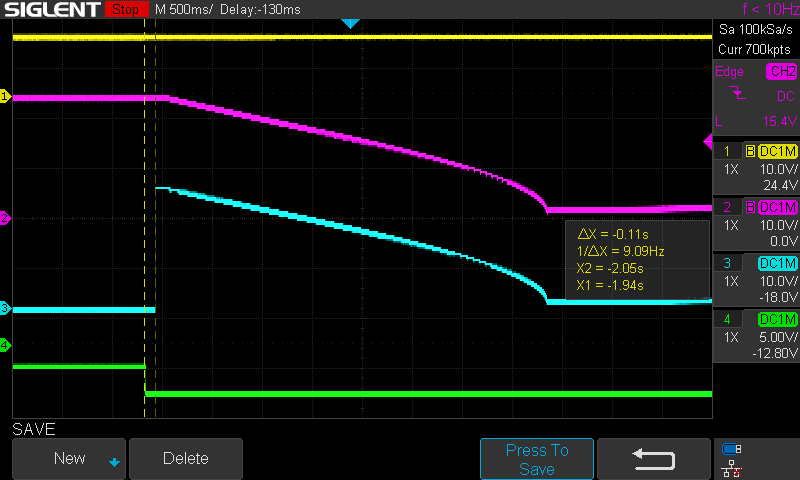
\includegraphics[width=0.9\textwidth]{pictures/cap_load_off.png}\hspace{1cm}
    \caption{Sistēmas ieslēgšanās oscilogramma ar testa lauktanzistoru un filtra kondensatoru}
\end{figure}
3.6. un 3.7. att. var redzēt sistēmas izslēgšanās procesu. Kad tiek saņemta komanda mikrokontrollierī par sistēmas atslēgšanu, tad RF jaudas pastiprinātājam tiek aizvērts, un pēc 100 milisekundēm aizvērts ieslēgšanas / izslēgšanas slēdzis un izslēgts 24 V industriālais barošanas avots.
\begin{figure}[H]
	\centering
    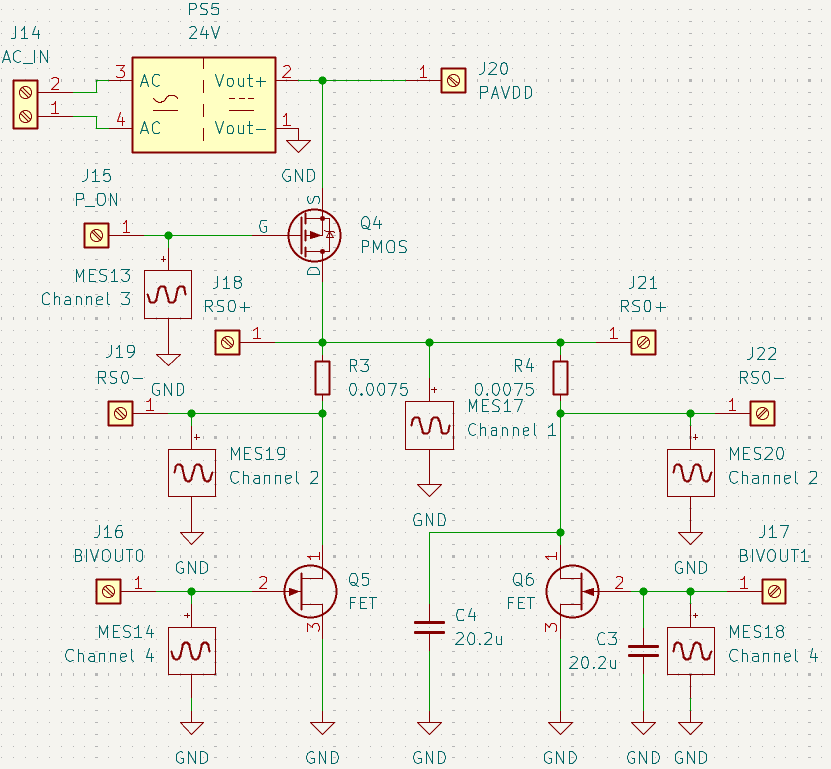
\includegraphics[width=0.8\textwidth]{pictures/test_diagram4.png}\hspace{1cm}
    \caption{Darba punkta iestatīšanas/atiestatīšanas testa diagramma ar differenciālo pāri}
\end{figure}
3.8. att. 1. un 2. kanāls veido diferenciālo pāri, kur tiek mērīts šunta rezistora sprieguma kritums, 3. kanāls mēra vadības signālu ieslēgšanas/izslēgšanas slēdzim un 4. kanāls aizvara spriegumu jaudas pastiprinātājam.
\begin{figure}[H]
	\centering
    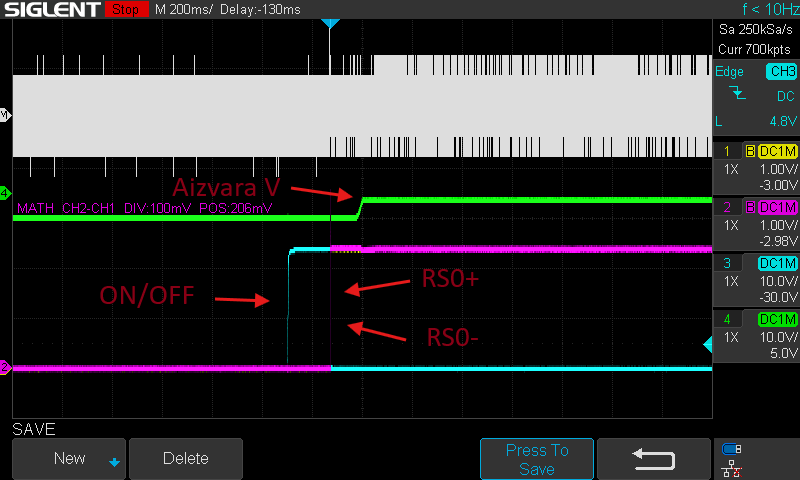
\includegraphics[width=0.9\textwidth]{pictures/current.png}\hspace{1cm}
    \caption{Sprieguma krituma noteikšana uz šunta rezistora}
\end{figure}
 Osciloskopam mazākajā mērīšanas diapazonā ir mazāki kanāla trokšņi, tāpēc osciloskopa tausti tika iestatīti uz 10x un osciloskopā nokonfigurēts uz 1x, lai varētu mērīt lielāku signālu ar mazāku sprieguma diapazonu, bet, neskatoties uz to, 1V mērīšanas diapozonam ir 100 mV pk-pk troksnis, tādēļ nebija iespējams izmērīt 22 mV sprieguma kritumu uz šunta rezistora, bet, kad beidzas pārejas process, tad var redzēt, ka troksnis sāk svārstīties ap citu vērtību, bet tas nedod noteiktu vērtību.